% This is a basic Math Paper

\documentclass[11pt]{article}

% Preamble

\usepackage[margin=1in]{geometry}
\usepackage{amsfonts, amsmath, amssymb}
\usepackage{fancyhdr, float, graphicx}
\usepackage[utf8]{inputenc} % Required for inputting international characters
\usepackage[T1]{fontenc} % Output font encoding for international characters
\usepackage{fouriernc} % Use the New Century Schoolbook font
\usepackage[nottoc, notlot, notlof]{tocbibind}
\usepackage{url}

% Header and Footer
\pagestyle{fancy}
\fancyhead{}
\fancyfoot{}
\fancyhead[L]{\textit{\Large{3D Glasses and Photo-elasticity}}}
%\fancyhead[R]{\textit{something}}
\fancyfoot[C]{\thepage}
\renewcommand{\footrulewidth}{1pt}



% Other Doc Editing
% \parindent 0ex
%\renewcommand{\baselinestretch}{1.5}

\begin{document}
	
	\begin{titlepage} 
		\centering 
		
		%---------------------------NAMES-------------------------------
		
		\huge\textsc{
			MIT World Peace University
		}\\
	
		\vspace{0.75\baselineskip} % space after Uni Name
		
		\LARGE{
			Engineering Physics\\
			First Year B. Tech, Trimester 3\\
			Academic Year 2021-22
		}
		
		\vfill % space after Sub Name
		
		%--------------------------TITLE-------------------------------
		
		\rule{\textwidth}{1.6pt}\vspace*{-\baselineskip}\vspace*{2pt}
		\rule{\textwidth}{0.6pt}
		\vspace{0.75\baselineskip} % Whitespace above the title
		
		
		
		\huge{\textsc{
				Understanding Photo-Elasticity and the Working of 3D Glasses
			}} \\
		
		
		
		\vspace{0.5\baselineskip} % Whitespace below the title
		\rule{\textwidth}{0.6pt}\vspace*{-\baselineskip}\vspace*{2.8pt}
		\rule{\textwidth}{1.6pt}
		
		\vspace{1\baselineskip} % Whitespace after the title block

		%--------------------------SUBTITLE --------------------------	
			
		\LARGE\textsc{
			Physics Assignment 1
		} % Subtitle or further description
		\vfill
		
		%--------------------------AUTHOR-------------------------------
		
		Prepared By
		\vspace{0.5\baselineskip} % Whitespace before the editors
		
		\Large{
			109054. Krishnaraj Thadesar
						
			Division 9 Batch I3
		}
		
		
		\vspace{0.5\baselineskip} % Whitespace below the editor list
		\today

	\end{titlepage}
	
\tableofcontents
\clearpage

\section{Introduction}
In the following assignment, we will try to understand how 3D glasses work, why they work, why they were invented, and the Physics behind it. We will also learn about Photo-Elasticity, understand the concept, and its applications. Let us begin with hte working of 3D Glasses. 

\section{The Human Eye}
To understand fully why every component of the 3D glass works, we have to understand how the Human eye perceives vision. \\
We have what is called \textit{sterioscopic vision}.
\subsection{Sterioscopic Vision}
Taken literally, stereoscopic vision describes the ability of the visual brain to register a sense of three-dimensional shape and form from visual inputs. In current usage, stereoscopic vision often refers uniquely to the sense of depth derived from the two eyes.\\

This means that Both of our eyes see the world as a 2D image. The images formed by both the eyes are slightly off. We can observe this by placing our thumb in front of our eyes and looking at it with only one eye. As we switch the eyes, we can see the position of your thumb shifting. These two images are interpreted by the brain, and it senses the depth of objects. So, basically, our brain takes two 2D images from our eyes and interprets them as 3D.\\

Each eye is like a camera that takes in a simple 2D image. So technically, you must not be able to perceive depth with just one eye. And it is in fact true to some extent. If we close one eye, and try to look into the distance and maybe calculate which building is farther and which is closer, it will be difficult, but looking with 2 eyes will make it better and easier. \\

But for everyday objects, this is not the case, as things like shadows and the fact that an object appears bigger if it is closer and smaller if it is far helps the brain determine whether the depth of field of the Object in question. \\

\subsection{How the brain makes 3D}

So basically our brain is what does the processing, it takes 2 images from our eyes as input, images that are approximately viewed from 2 different perspectives, set on average 7.5 cm apart (Human Average distance between 2 eyes), and it merges them to \textbf{make us believe that we are looking at a 3 Dimensional Object.}\\

The problem then with movies, images, paper, and screens is that they are flat and can only therefore appear 2D to us. So as to make it real, we must then find a way to somehow feed the brain what it expects to make a 3D image. \textbf{\textit{\textit{It takes as input 2 2D images, as seen from 2 different perspectives set 7.5 cm apart, and makes us think we are looking at something 3D}}}

\section{The Beginning of 3D Movies - Separation by Colors}

\subsection{Working}

\begin{figure}[H]
	\centering
	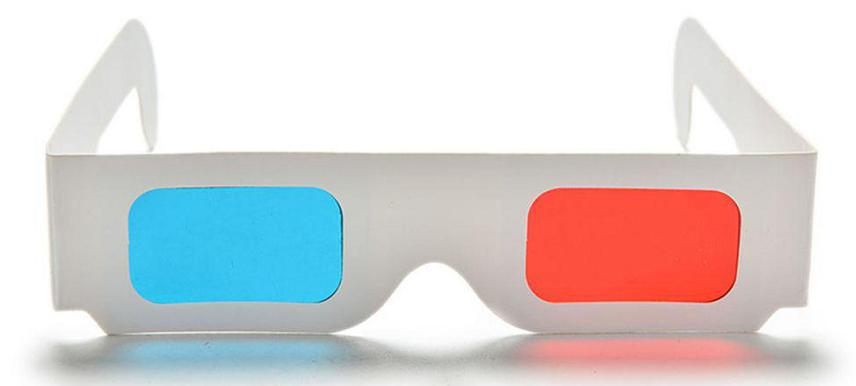
\includegraphics[scale=.25]{Color 3D Glass.jpg}
	\caption{A Simple 3D Glass with color filters.}
	\label{fig:This figure}
\end{figure}

So as soon as we figured out that all we need is 2 perspectives, filmmakers could now just shoot their film with 2 camera angles, kept about 7.5cm apart, and have 2 copies of the same scenes, but shot twice.\\ 

They would now put color filters, so that one would have only blue and the other would have only red. Then we would wear glasses as shown above, where the blue filter would let the red light in, which was intended for the right eye, and the red filter would let the blue light in which was intended for the left eye.\\ 

So now there are 2 separate 2D images with different perspectives, and so the brain produced the 3D effect required. 

\subsection{3D Images for such glasses}
\begin{figure}[H]
	\centering
	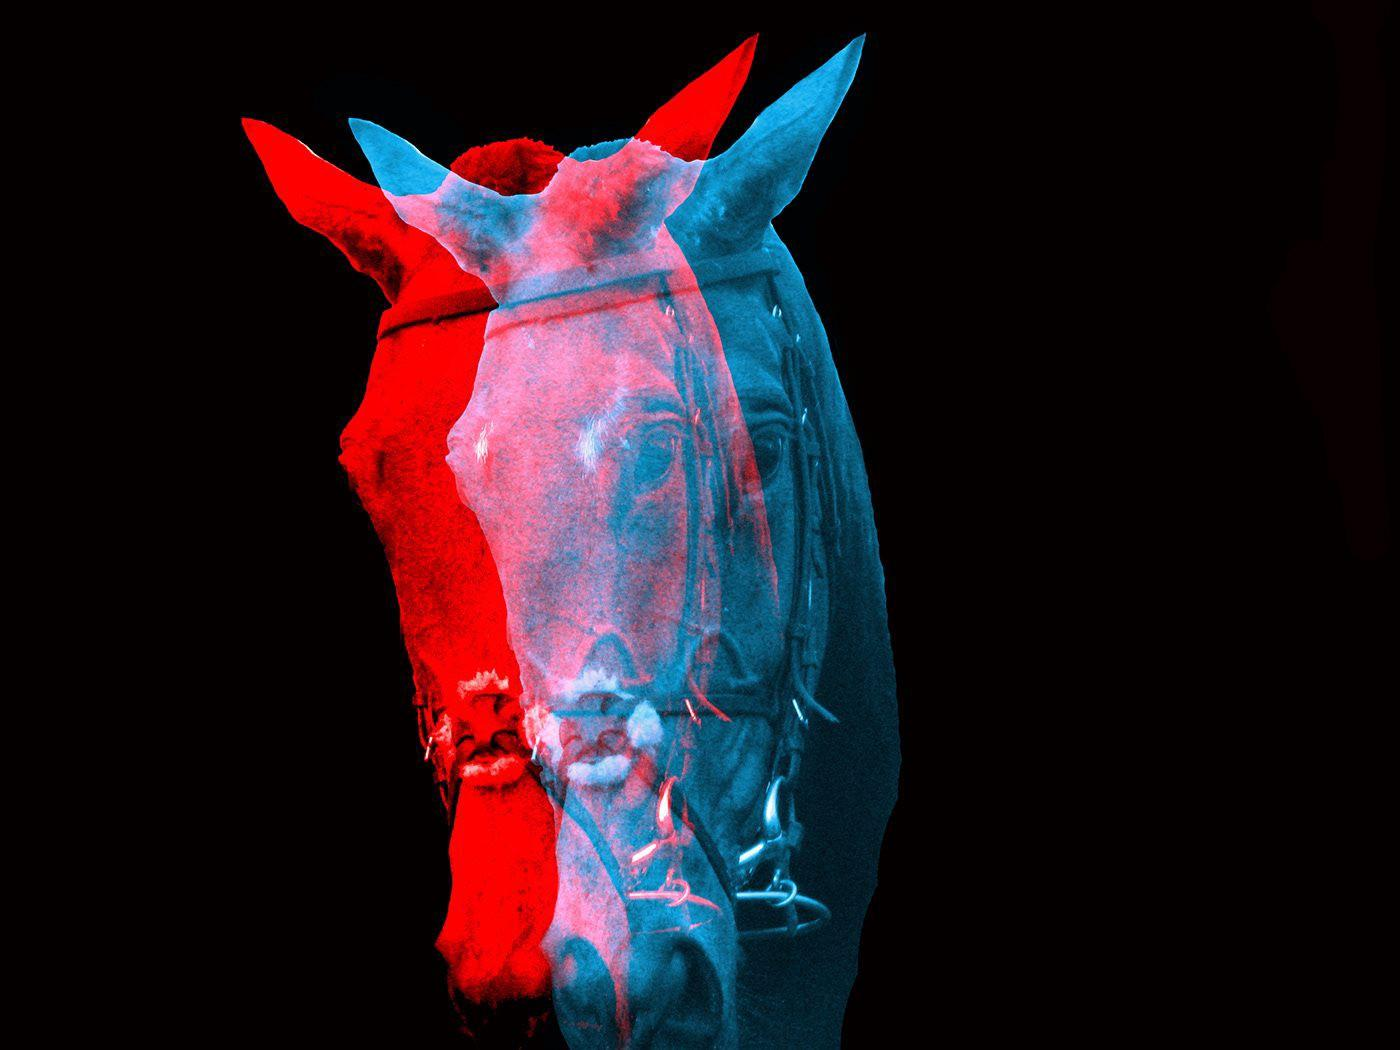
\includegraphics[scale=.15]{3D Glasses working 2.jpg}
	\caption{This is how the image would look without the glasses.}
	\label{fig:This figure}
\end{figure}
\subsection{The Drawback}
The blue filter blocked all the blue light, and the red filter blocked all the red light. Due to this, now the movie could not be enjoyed in its true color, which was more important than the 3D aspect of the movie, and so we were forced to find a better method. 

\section{The Better Method: Using Linear Polarization}

\subsection{Working}

New Glasses would now be made using polarized light, to counter the problems with color. The aim was always the same, to produce 2 different perspective 2D images, separated by 7.5cm. Now we know that filming like this on 2 different cameras was possible and simple enough.\\

But Polarized light has the advantage that all colors of the film could be polarized along a single axis, and our eyes wouldnt know as we arent sensitive to polarization of light. Our brain cannot differentiate between polarized and unpolarized light. The loss of intensity could be brought up digitally. \\

It was the perfect solution to pass vertically aligned linearly polarized light for the left eye with one projector, and horizontally aligned linearly polarized light for the right eye with another project kept next to it.\\

The Glasses would then just have the same polarization axis, horizontal for left and vertical for right. The horizontally polarized light wouldnt pass through the right eye, and vice versa for left. So now you could see the movie's full colors. 

\begin{figure}[H]
	\centering
	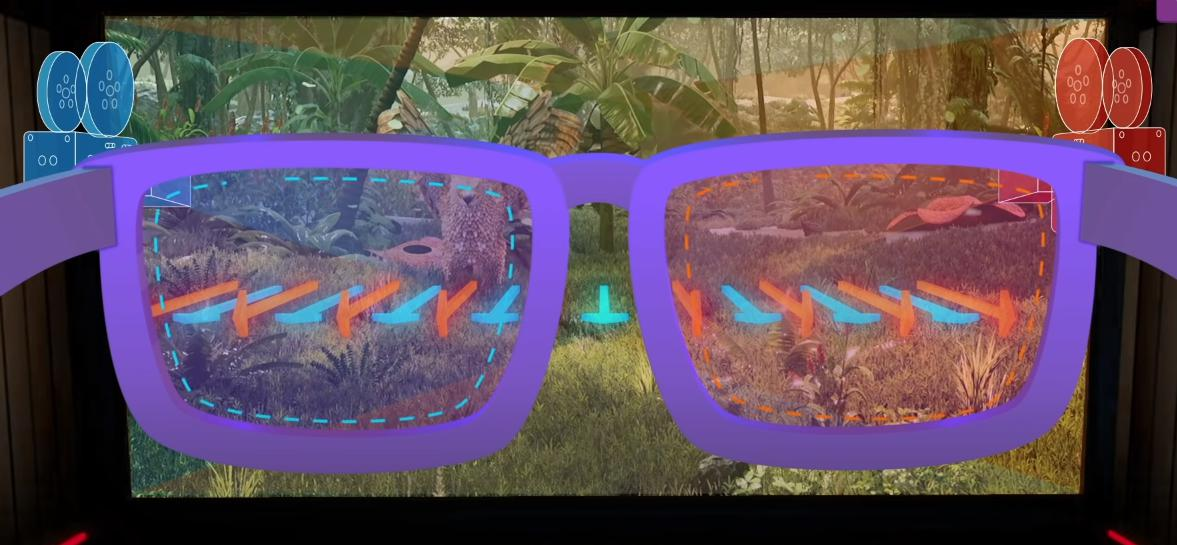
\includegraphics[scale=.37]{method 2.jpg}
	\caption{How linearly polarized light could be used to make 3D images.}
	\label{fig:This figure}
\end{figure}

\subsection{The Drawback}
The drawback in this case is what one would expect. If the person watching the movie tilts his or her head, then the entire axis of the glasses shifts depending on the tilt angle. This would drastically (in accordance with Law of Malus) reduce the intensity of light reaching his or her eyes.
\begin{equation}
 I_\theta = I_m cos^2\theta
\end{equation}
It is not possible to sit for long periods of time without tilting your head, and so another solution was required. 

\section{The Best Method: Using Circularly Polarized Light}
\subsection{Working}

To counter this problem, the glasses needed to have circular polarizers instead of linear. A light wave can have only two types of circular polarization — clockwise and counterclockwise. Just like linear polarizers, circular polarizers allow only one of these to pass. This is the method in use today. 
\begin{figure}[H]
	\centering
	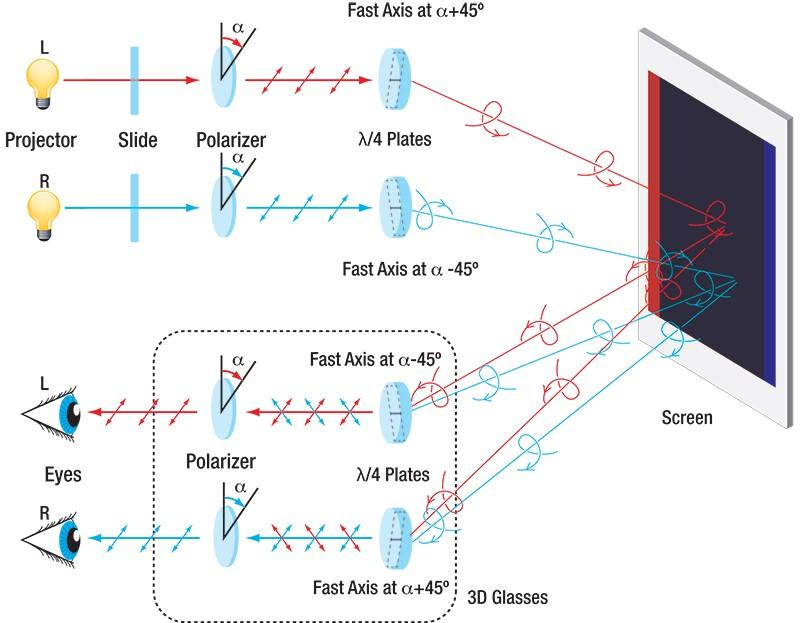
\includegraphics[scale=.5]{method 3.jpg}
	\caption{How circularly polarized light could be used to make 3D images.}
	\label{fig:This figure}
\end{figure}
So, the movie makers make the same two images for the 3D glasses, but this time using light with clockwise and counterclockwise polarizations. The 3D glasses have one clockwise polarizer and one counterclockwise polariser, ensuring two different images for each eye. This would allow for images with proper original colour and also made sure that the viewer could view the same image even with a tilted head, as a clockwise polarized wave is still clockwise even if the viewer tilts his/her head.

\section{Other Applications}
\begin{figure}[H]
	\centering
	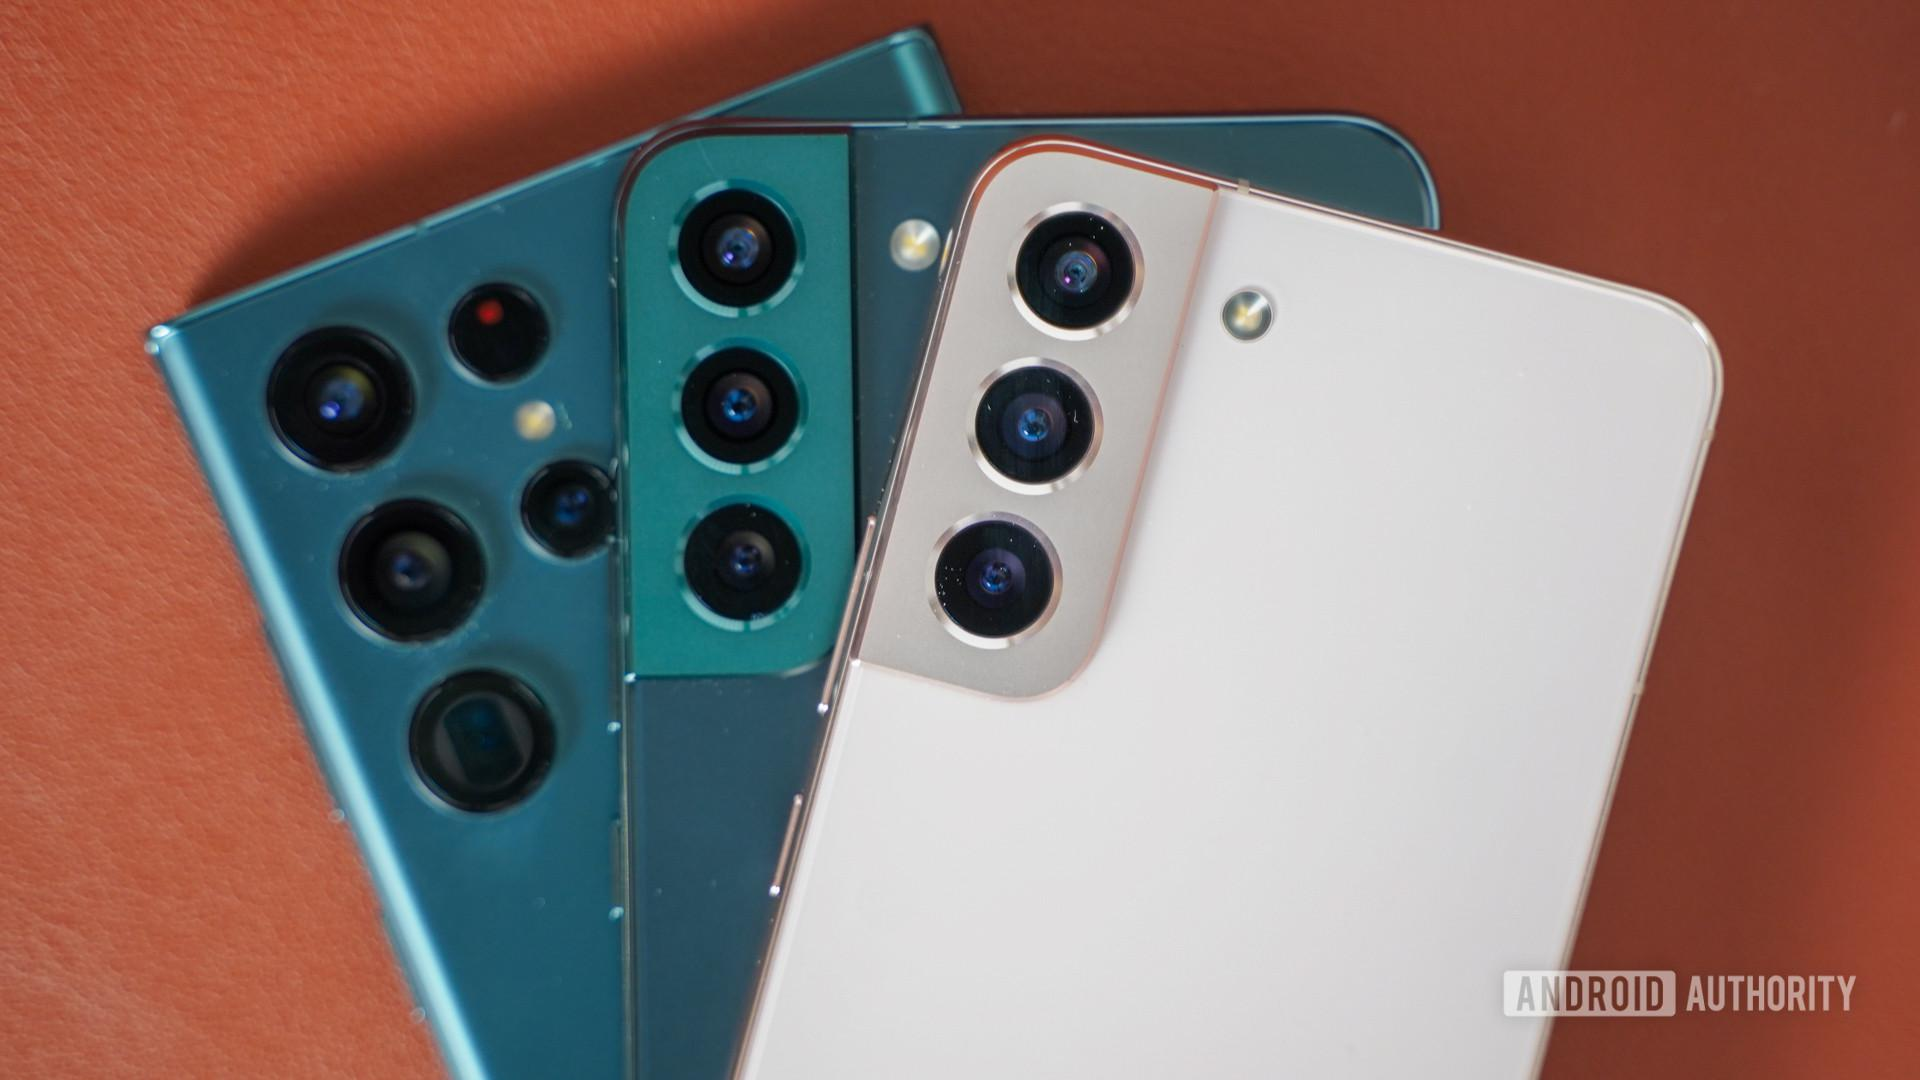
\includegraphics[scale=.2]{phone cameras.jpg}
	\caption{Why cell phones now have multiple cameras}
	\label{fig:This figure}
\end{figure}

A common trend now is the availability of \textit{multiple cameras} on cell phones. The logic behind them is also the same as that of our eyes. If you were to focus on a particular object with your eyes, then you will find that the background behind that object acquires a natural blur caused by lack of focus.\\

The same can happen with one camera focusing on a single object, but by using 2 or more such cameras, you could replicate the effect made by our eyes, and will therefore achieve a more real and natural looking image as opposed to ones taken from 1 camera.\\

It is not that such technology, equations, algorithms or methods did not exist prior to the trend, it is simple that the processors we used till now were not powerful and fast enough to carry out those algorithms thousands of times a second to show a live preview of such background blur (\textit{calculations our brain naturally does}). Now that we have faster processors, it is possible to apply such features.

\section{Photo-Elasticity}

The words Photo and Elasticity dont often go hand in hand as one is related to properties of light, and the latter often deals with matter, and its interactions with its surroundings under the influence of forces. So it is interesting to see how they could both be related to each other. 

\subsection{Discovery}
The photoelastic phenomenon was first discovered by the Scottish physicist David Brewster, who immediately recognized it as stress-induced birefringence. That diagnosis was confirmed in a direct refraction experiment by Augustin-Jean Fresnel.

\subsection{Birefringence}
Birefringence is the optical property of a material having a refractive index that depends on the polarization and propagation direction of light. These optically anisotropic materials are said to be birefringent (or birefractive).

\subsection{Definition}
Photoelasticity describes changes in the optical properties of a material under mechanical deformation. It is a property of all dielectric media and is often used to experimentally determine the stress distribution in a material, where it gives a picture of stress distributions around discontinuities in materials. It is the effect that an isotropic material can become birefringent(anisotropic) when placed under stress. \\

\begin{equation}
\text{Induced birefringence} \propto \text{Stress}
\end{equation}


\begin{figure}[H]
	\centering
	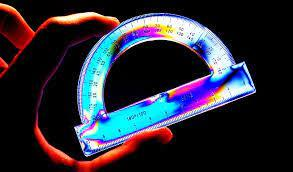
\includegraphics[scale=.9]{photoelasticity protractor.jpg}
	\centering
	\caption{Photoelasticity showing the stress in the protractor, could be due to cooling method}
	\label{fig:This figure}
\end{figure}

\subsection{Applications}
\begin{enumerate}
	\item Photoelasticity has been used for a variety of stress analyses
	\item Use in design, particularly before the discovery of numerical methods, which would then lead to computerized replacement of photoelastic experiments
	\item Digitization of polariscopy enables fast image acquisition and data processing, which allows its industrial applications to control quality of manufacturing process for materials such as glass and polymer.
	\item Dentistry utilizes photoelasticity to analyze strain in denture materials.
	\item Silicone Wafer Stress Analysis
	\item We can make models of infrastructure that are transparent and use them to see the levels of stress at each point.
	\begin{figure}[H]
		\centering
		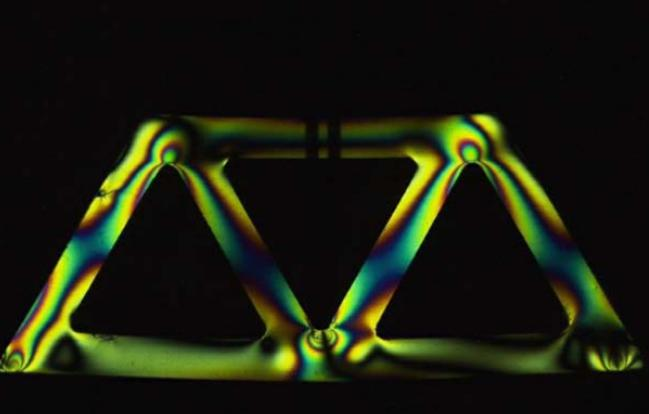
\includegraphics[scale=.5]{bridge.jpg}
		\centering
		\caption{A model of a bridge structure showing points of stress using photoelasticity}
		\label{fig:This figure}
	\end{figure} 
\end{enumerate}

\begin{figure}[H]
	\centering
	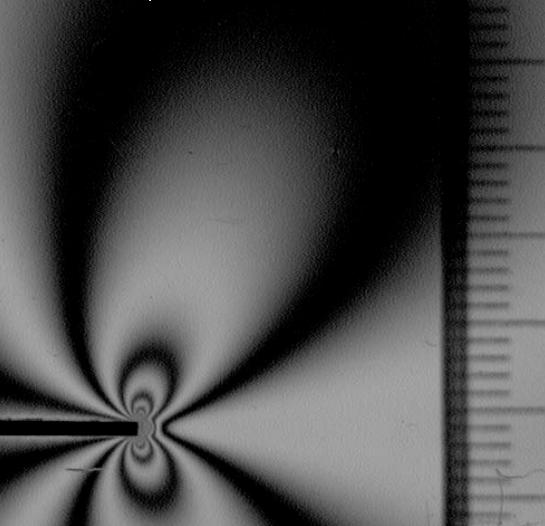
\includegraphics[scale=.5]{mono photo elasticity.jpg}
	\centering
	\caption{Better definition of fringes using a monochromatic light source}
	\label{fig:This figure}
\end{figure}

\begin{figure}[H]
	\centering
	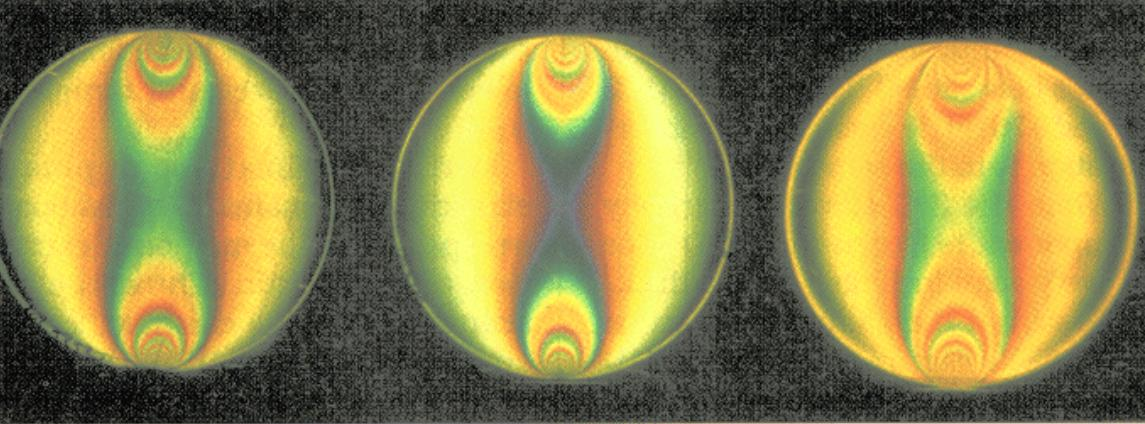
\includegraphics[scale=.4]{si wafer analysis.jpg}
	\centering
	\caption{Analysis of Silicone Wafers using Photoelasticity}
	\label{fig:This figure}
\end{figure}

\section{Conclusion}
I have learnt in detail about 3D glasses, their working, their history, and the physics that goes behind the production of a simple yet fascinating product. The use of circular polarized light was understood thoroughly. \\

Photo-Elasticity is a very cool application of polarization, and it was also understood, although not so much in depth, as the detailed structure of molecules that change their behaviour from isotropic to anisotropic goes beyond the scope of my understanding. But its application was studied and understood in detail. 


\clearpage
\begin{thebibliography}{}
	
	\bibitem{How do 3D glasses work?}
	"How do 3D glasses work?"\\
	\url{https://www.youtube.com/watch?v=c9ew1J0PY-M}

	\bibitem{sth}
	"How do 3D Glasses Work?"\\
	\url{https://medium.com/illumination/how-do-3d-glasses-work-12304df48757}
		
	\bibitem{sth1}
	"Sterioscopic Vision"\\
	\url{https://www.sciencedirect.com/topics/medicine-and-dentistry/stereoscopic-vision}
	
	\bibitem{sth2}
	"Photoelasticity"\\
	\url{https://www.youtube.com/watch?v=koaRyPnLjBg&t=301s}
	
	
\end{thebibliography}
	
\end{document}